\newpage
\section{Äquivalenzumformungen}

% ------------------------------------------------------------------------------
\subsection{Begriff}
Gleichungen dürfen nur nach bestimmten Regeln umgeformt werden, sodass die resultierende Gleichung \textbf{äquivalent} zur Ausgangsgleichung ist.

Eine Gleichung kann man sich als Balkenwaage vorstellen. Wenn die Gleichung eine wahre Aussage ist, sind die beiden Seiten ausbalanciert. Es sind nur solche Veränderungen erlaubt, welche die Balance der Waage erhalten.
\begin{center}
  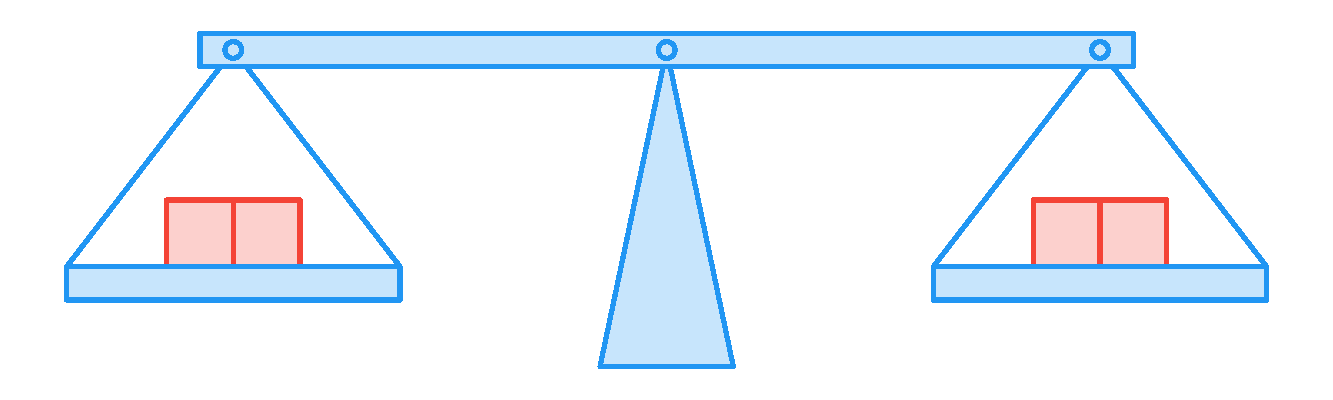
\includegraphics[height=4cm]{Waage.pdf}
\end{center}

Anhand der wage kann man sich überlegen, welche Änderungen erlaubt sind:

\begin{itemize}
  \item eine Seite umschichten
  \item auf beiden Seiten das Gleiche hinzufügen oder entfernen
  \item beide Seiten verdoppeln oder halbieren
  \item beide Seiten vertauschen
\end{itemize}

Genau so können auch Gleichungen umgeformt werden:

\begin{itemize}
  \item Die Terme auf jeder Seite der Gleichung dürfen umgeformt werden (siehe Termumformungen).
  \item Auf beiden Seiten einer Gleichung kann der gleiche Term addiert oder subtrahiert werden.
  \item Beide Seiten einer Gleichung können mit dem gleichen Term multipliziert oder dividiert werden.
  \item Die beiden Seiten einer Gleichung dürfen vertauscht werden.
\end{itemize}

% ------------------------------------------------------------------------------
\subsection{Umformungsprotokoll}

Damit die an einer Gleichung vorgenommen Umformungen nachvollzogen werden können, wird ein \textbf{Umformungsprotokoll} geführt. Dazu wird rechts der Gleichung, durch eine vertikale Linie abgetrennt, jeweils der Umformungsschritt angegeben.
\[\def\arraystretch{2}\begin{eqt}
  2x+6 &= 0  & -6 \\
    2x &= -6 & :2 \\
     x &= -\frac{6}{2} & \text{kürzen} \\
     x &= -3
\end{eqt}\]

% ------------------------------------------------------------------------------
\subsection{Terme umformen}

Auf jeder Seite der Gleichung befindet sich ein Term. Diese dürfen mit den bekannten Regeln umgeformt werden.

\begin{example}
  \textbf{Beispiel:} Hier werden die Terme auf beiden Seiten zunächst ausmultipliziert. Danach werden auf der linken Seite die Summanden zusammengefasst.
  \[\begin{eqt}
      (2x-1)(3+2x) &= 4x(x-5)    & \text{ausmultiplizieren} \\
    6x+4x^{2}-3-2x &= 4x^{2}-20x & \text{zusammenfassen} \\
       4x^{2}+4x-3 &= 4x^{2}-20x
  \end{eqt}\]
\end{example}

% ------------------------------------------------------------------------------
\subsection{Addieren oder Subtrahieren eines Terms}

Auf beiden Seiten der Gleichung darf der gleiche Term addiert oder subtrahiert werden. Dabei wird der Term auf beiden Seiten der Gleichung an den vorhandenen Term angefügt. Anschliessend können die Summanden auf beiden Seiten zusammengefasst werden.

\begin{example}
  \textbf{Beispiel:} Hier wird auf beiden Seiten der Gleichung $4x^{2}$ und $4x$ subtrahiert. Damit wird $x^{2}$ vollständig aus der Gleichung entfernt und $x$ auf die rechte Seite der Gleichung gebracht.
  \[\begin{eqt}
    4x^{2}+4x-3 &= 4x^{2}-20x & -4x^{2}-4x \\
    4x^{2}+4x-3\mathcolor{red}{-x^{2}-4x} &= 4x^{2}-20x\mathcolor{red}{-x^{2}-4x} & \text{zusammenfassen} \\
             -3 &= -24x
  \end{eqt}\]
\end{example}

% ------------------------------------------------------------------------------
\subsection{Multiplizieren oder Dividieren mit einem Term}

Beide Seiten der Gleichung dürfen mit dem gleichen Term multipliziert oder dividiert werden. Dabei muss dieser \textbf{ungleich Null} sein. Dabei wird \textbf{jeder Summand} auf beiden Seiten der Gleichung mit dem Term multipliziert beziehungsweise durch ihn dividiert.

\begin{example}
  \textbf{Beispiel:} Hier werden beide Seiten der Gleichung mit dem kgV der Nenner multipliziert, um Brüche zu entfernen.
  \[\begin{eqt}
    \frac{x}{4}+\frac{1}{5} &= \frac{x}{2}+\frac{x}{6}                 & \cdot \kgV(4,5,2,6) = 60 \\[4mm]
    \frac{\mathcolor{red}{60\cdot} x}{4}+\frac{\mathcolor{red}{60\cdot} 1}{5} &= \frac{\mathcolor{red}{60\cdot} x}{2}+\frac{\mathcolor{red}{60\cdot} x}{6} & \text{kürzen} \\[3mm]
    15x+12 &= 30x+10x
  \end{eqt}\]
\end{example}


\begin{example}
  \textbf{Beispiel:} Hier werden beide Seiten der Gleichung mit $-1$ multipliziert, um die negativen Vorzeichen zu entfernen.
  Anschliessend werden beide Seiten der Gleichung durch $24$ dividiert, um die Variable $x$ vollständig zu isolieren.
  \[\begin{eqt}
    -3 &= -24x & \cdot(-1) \\
    \textcolor{red}{(-1)\cdot}(-3) &= \textcolor{red}{(-1)\cdot}(-24x)\ & \text{Klammern ausrechnen} \\
             3 &= 24x
  \end{eqt}\]
\end{example}

Ist auf einer Seite der Gleichung ein Mehrfaches der Variable vorhanden, so kann die Gleichung durch diesen Faktor dividiert werden, um die Variable zu isolieren. Dabei wird jeder Summand auf beiden Seiten der Gleichung durch den Faktor dividiert. Anschliessend kann gekürzt werden:

\begin{example}
  \textbf{Beispiel:} Hier werden beide Seiten der Gleichung durch $24$ dividiert, um die Variable $x$ vollständig zu isolieren.
  \[\begin{eqt}
    3 &= 24x  & :24 \\[3mm]
    \frac{3}{\textcolor{red}{24}} &= \frac{24x}{\textcolor{red}{24}} & \text{kürzen} \\[4mm]
    \frac{1}{8} &= x
  \end{eqt}\]
\end{example}
